\documentclass[../../../Main.tex]{subfiles}
\begin{document}
\subsection*{Few Terminologies}
\begin{enumerate}
    \item \textbf{Heat and energy.} Heat is considered a form of energy. It can be converted to work, and in turn can be produced by consuming work. Work and heat together obey law of conservation of energy.
    \item \textbf{Thermodynamic equilibrium.} The state of a thermodynamic system which does not change with time is called the state of thermodynamic equilibrium.
    \item \textbf{State variable.} The state variables--such as pressure $P$, volume $V$, and temperature $T$--in the state of equilibrium are not independent. The relationship between them is known as the equation of state.
    \item \textbf{Thermodynamic transformation.} The state of a system chan-ges when the external conditions are changed. When its state changes, the system is said to undergo thermodynamic transformation.
    \item \textbf{Quasi-static.} If the state variables change so slowly that the system can be assumed to be in thermodynamic equilibrium at any instant then the transformation of the system is said to be quasi-static.
    \item \textbf{Reversible and irreversible.} If the transformation is carried such that it is possible to retrace the steps from its final to the initial state by reversing the external conditions then it is called reversible. Else the transformation is called irreversible.
    \item \textbf{Isolated system.} A system enclosed by partition such that no exchange of volume, mole number, heat or work is possible.
    \item \textbf{Simple system.} A system which is microscopically homogeneous, isotropic, electrically neutral, and not under external force.
    \item \textbf{Composite system} A system consisting two or more subsystems.
    \item \textbf{Adiabatic system.} If the transformation is such that the system does not exchange heat with its surroundings then the transformation is said to be adiabatic.
    \item \textbf{Isothermal.} A transformation in which temperature of the system remains unchanged is called isothermal.
    \item \textbf{Isobaric.} A transformation in which pressure of the system remains unchanged is called
    isobaric.
    \item \textbf{Heat reservoir.} A thermal or heat reservoir is a system so large that addition or removal of a finite amount of heat from it does not change its temperature.
    \item \textbf{Cyclic transformation.} If a transformation is such that it restores the system to its initial state then it is called cyclic. 
\end{enumerate}

\subsection*{The Ideal Gas} 
The ideal gas model represents the gas particles as point particles (i.e. a material body having mass but no spatial extent), and assumes that there are no (attractive or repulsive) physical interactions between them. For an ideal gas composed of $N$ particles or $n$ moles in equilibrium, the pressure $P$ is related with the volume $V$ occupied by the gas and its temperature $T$, through the ideal gas equation:
\begin{equation*}
    P V = n RT = N k_B T
\end{equation*}
where $R=8.315$ joule/mole K $k_B = 1.38 \times 10^{-16}$ erg/K. The ideal gas equation was stated in 1834 by Benoit Emile Clapeyron (1799-1864) and results from combining the old gas laws: 
\begin{enumerate}
    \item \textbf{Boyle's law.} If temperature is kept constant, the pressure is proportional to the density, $P\propto \rho$. 
    \item \textbf{Amonton's law.} If volume is kept constant, the pressure is proportional to the temperature, $V\propto T$.
    \item \textbf{Gay-Lussac' law.} If pressure is kept constant, the volume is proportional to the temperature, $V\propto T$
\end{enumerate}

\subsubsection*{Van der Waals Equation of State.} The equation of state for a real gas derived by van der Waals was also based on the kinetic theory and the Virial theorem. Here we give standard phenomenological derivation of the equation, obtained by introducing following modifications in the ideal gas law:
\begin{enumerate}
    \item \textbf{Specific volume.} It is assumed that the molecules are not point particles but are hard spheres. This results in each molecule excluding some volume, say $b$, from the total volume $V$. It was argued that the ideal gas law should therefore be modified to replace $V$ by $V - N b$.
    \item \textbf{Force of attraction.} The molecules attract each other when separated by distances greater than the molecular radius $r_0$. Assuming that the molecules are distributed uniformly, each mole-cule in the interior is acted upon by forces on all sides resulting in net-zero force; however near the boundary surfaces therefore experience a net inward force resulting in reduction of pressure. This causes net reduction of pressure proportional to $(N /V )^2$ which must be subtracted from the pressure appearing in the ideal gas law.
\end{enumerate}
Under the suggested modifications, the ideal gas law assumes the form
\begin{equation*}
    P=\frac{Nk_B T}{V-Nb}-\frac{a}{(V/N)^2}=\frac{k_BT}{v-b}- \frac{a}{v^2}
\end{equation*}
where $v=V/N$ is the specific volume. Since, in addition to the equation of state relating pressure, volume, and temperature, complete description of thermodynamic properties requires also the knowledge of its internal energy as a function of the state variables, we give (without the derivation)
\begin{equation*}
    u=ck_BT-\frac{a}{v}
\end{equation*}

\subsubsection*{Entropy of ideal gas.} Consider a reversible process which takes $N$ molecules of an ideal gas be in equilibrium in the state $A$ to the equilibrium state $B$. The process being reversible is described by the form of the first law which, on reversible process takes the form of 
\begin{eqnarray}
    dU=T\;dS-P\;dV
\end{eqnarray}
Solving for the entropy
\begin{eqnarray}
    dS=\frac{dT}{T}+\frac{P}{T}dV
\end{eqnarray}
Considering $T$ can be written as
\begin{equation*}
    T=\frac{PV}{Nk_B}=\frac{U}{cNk_B}
\end{equation*}
then 
\begin{equation*}
    dS=Nk_B\biggl(c\frac{dU}{U}+\frac{dV}{V}\biggr)
\end{equation*}
On integrating the equation above, we get
\begin{equation*}
    S=nK_B\bigl[c\ln U+\ln V\bigr]+K
\end{equation*}
where $K$ is the integration constant. Determination of absolute value of entropy in a state would, of course, require knowledge of $K$. However, it plays no role in computing entropy change in going from state $A$ to state $B$ as in that case
\begin{equation*}
    S(B)-S(A)=Nk_B \biggl[c\ln\frac{U_B}{U_A}+\ln\frac{V_B}{V_A}\biggr]
\end{equation*}

\subsection*{Carnot Engine}
\begin{figure*}
    \centering
    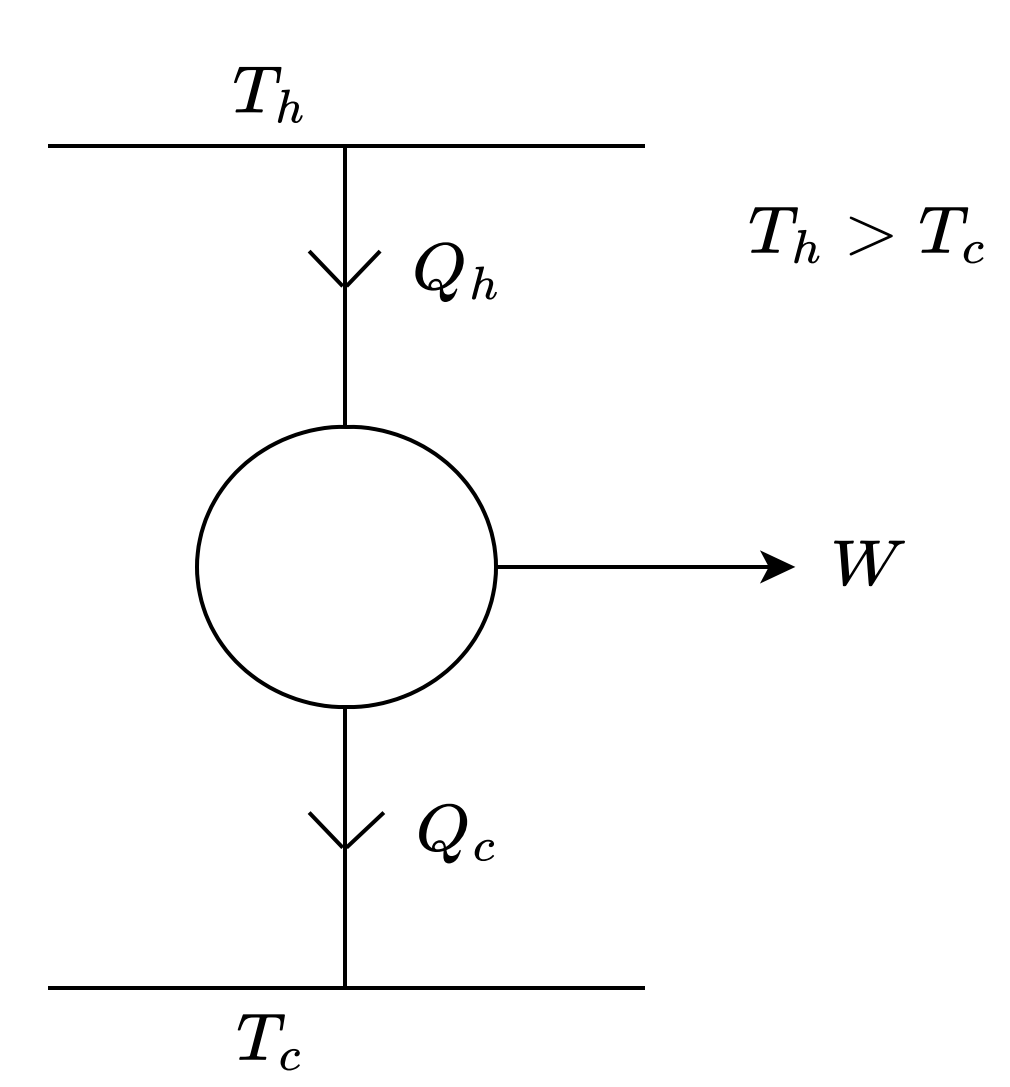
\includegraphics[width=0.4\textwidth]{../../../Rss/Themodynamics/KeyConcepts/CarnotEngine.png}
    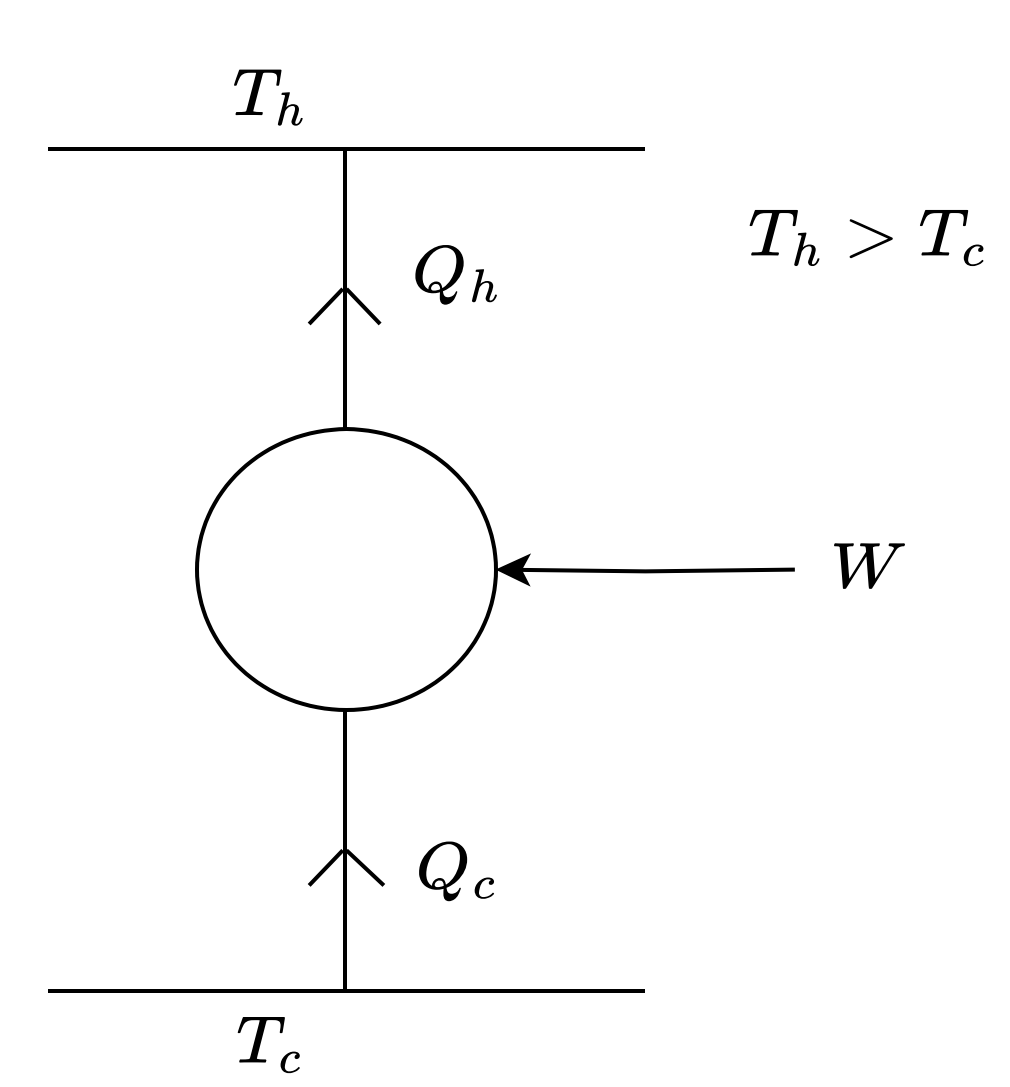
\includegraphics[width=0.4\textwidth]{../../../Rss/Themodynamics/KeyConcepts/ReverseCarnotEngine.png}
    \caption*{Figure: Carnot engine and reverse Carnot engine.}
\end{figure*}
The Carnot engine (or machine) is a theoretical heat engine envisioned by Sadi Carnot that operates a reversible cyclic process termed Carnot cycle.

If it is assumed that heat cannot be transported from a cold to a hot reservoir without doing any work then
\begin{enumerate}
    \item No engine is more efficient than reversible Carnot engine.
    \item All reversible Carnot engines operating between same reservoirs have same efficiency. 
\end{enumerate}

The work produced in one cycle of the process is the difference in the amount of heat absorbed and the heat--$W=Q_h-Q_c$. Hence, efficiency $\mu$ defined as the ratio of work $W$ produced by the engine to the amount of heat $Q_h$ received by it,
\begin{equation*}
    \mu=\frac{W}{Q_h}=1-\frac{Q_c }{Q_h}=1-\frac{T_c}{T_h}
\end{equation*}
where the last line is obtained from clever derivation. I won't go into the derivation itself, but one important part of the derivation also prove, for a reversible Carnot engine operating with any fluid and process, 
\begin{equation*}
    \frac{Q_h}{T_h}=\frac{Q_c}{T_c}
\end{equation*}
Also note that the $T$ in question is measure in kelvin, not Celsius. 

\subsubsection*{Cyclic Process.} Consider the cyclic process comprises a sequence of four reversible processes of a thermodynamic system, namely, an isothermal expansion, an adiabatic expansion, an isothermal compression, and an adiabatic compression. Suppose also that the working fluid is an ideal gas. Those processes are as follows.

\begin{enumerate}
    \item \textbf{Point A.} The gas is initially in equilibrium at temperature $T_h$ and its pressure and volume $P_A $, $V_A$. The temperature is kept constant by keeping the gas in contact with a heat reservoir at the desired temperature. The gas is then let to expand isothermally to volume $V_B$ with $P_B$ as its pressure.

    \item \textbf{Point B.} At $B$ the gas is isolated from the heat reservoir. The amount of heat absorbed along $A\rightarrow B$ may be evaluated using the first law $dU=\dbar Q-P\;dV$, along with the two equation of state $PV=Nk_BT$ and $U=cNk_BT$. Since the temperature has the constant value, $dU=0$. Therefore,
    \begin{equation*}
        dQ=Nk_BT_h  \frac{dV}{V}
    \end{equation*}
    Integrating between initial and final volumes
    \begin{equation*}
        Q_h=Nk_BT_h \ln \frac{V_B}{V_A}
    \end{equation*}

    The gas is then expands further but without exchanging heat with the environment, an adiabatic expansion. It continues till it volume and pressure become $V_C$ and $P_C$.

    \item \textbf{Point C.} At $C$ it is brought in contact with the reservoir at temperature $T_C$. First we consider the transformation of $B\rightarrow C$. Since it is adiabatic, it does not involve exchange of heat. The first law reads as
    \begin{align*}
        dU+P\;dV=0
    \end{align*}
    Now we use the equations of state 
    \begin{multline*}
        C_V\;dT+P\;dV\implies dT+\frac{P\;dV}{C_V}\implies\frac{dT}{T}+\frac{P\;dT}{cNk_BT}\\\implies \frac{dT}{T}+\frac{dV}{cV}\implies\frac{dT}{T}+(\gmto-1)\frac{dV}{V}
    \end{multline*}
    And we obtain
    \begin{equation*}
        \frac{dT}{T}+(\gmto-1)\frac{dV}{V}=0
    \end{equation*}
    On integrating the equation above between the state, we get 
    \begin{equation*}
        \ln \frac{T_C}{T_B}+(\gmto-1)\ln\frac{V_C}{V_B}=0
    \end{equation*}
    We can write 
    \begin{equation*}
        \ln \frac{T_C}{T_B}+(\gmto-1)\ln\frac{V_C}{V_B}=\ln \frac{T_C}{T_B}\frac{V_C^{\gmto-1}}{V_B^{\gmto-1}} 
    \end{equation*}
    which implies
    \begin{equation*}
        \frac{V_C^{\gmto-1}}{V_B^{\gmto-1}} =1
    \end{equation*}
    In other words
    \begin{equation*}
        TV^{\gmto-1}=\text{constant.}
    \end{equation*}
    Expressing $T$ in terms of $P$ and $V$
    \begin{equation*}
        PV^{\gmto-1}=\text{constant.}
    \end{equation*}
    And expressing $V$ in terms of $P$ and $T$
    \begin{equation*}
        TP^{-v}=\text{constant.}
    \end{equation*}
    where $v=(\gmto-1)/\gmto$. These equations are called \textbf{adiabatic equations of state.}

    Due to the reservoir $T_c$, the gas compresses isothermally till its volume and pressure become $V_D$, $P_D$.

    \item \textbf{Point D.} At $ D$ it is again isolated. As before, we consider the transformation of $C\rightarrow D$ first. Along $CD$, the temperature has the constant value $T_c$ and volume varies from $V_C$ to $V_D$ leads to the following expression for the heat \textbf{received} by the gas:
    \begin{equation*}
        Q'_C=Nk_BT_c\ln \frac{V_D}{V_C}
    \end{equation*}
    Since $V_D < V_D$, the heat absorbed by the gas is negative, which means that a positive amount of heat is delivered to the reservoir. Hence, the amount of heat delivered to the reservoir is 
    \begin{equation*}
        Q_C=-Q'_C=Nk_BT_c\ln\frac{V_C}{V_D}
    \end{equation*}
    
    The gas is then compressed adiabatically till its pressure, volume, and temperature attain their initial values $P_A$, $V_A$, and $T_h$. Also, since the process from $D$ to $A$ is adiabatic, no heat is exchanged with the surroundings. 
\end{enumerate}

\begin{figure*}
    \centering
    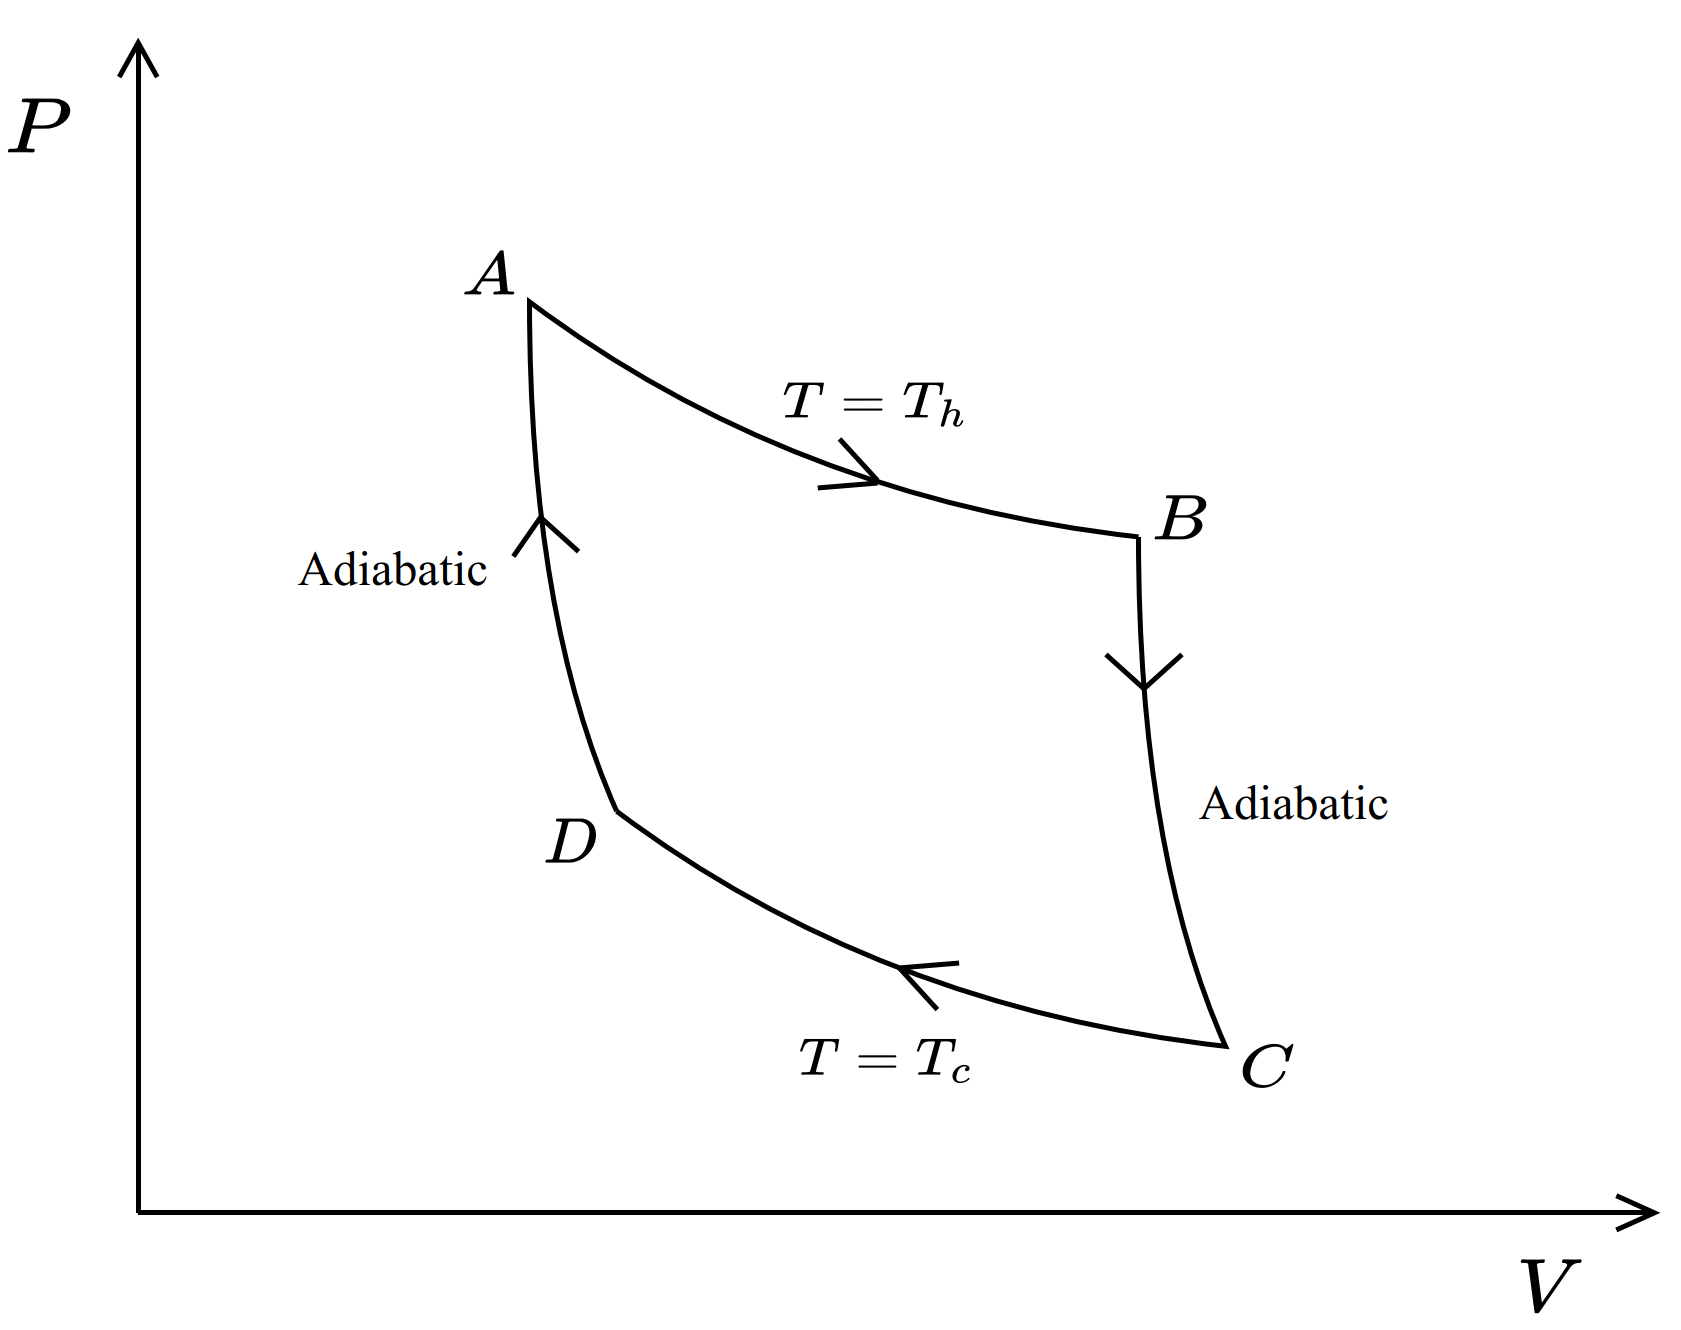
\includegraphics[width=0.5\textwidth]{../../../Rss/Themodynamics/KeyConcepts/CylicCarnot.png}
    \caption*{Figure: $PV$ diagram of a cyclic Carnot process.}
\end{figure*}

\subsubsection*{Carnot's equation in cyclic processes.} The Carnot's equation still holds true even in cyclic process. To prove this, first we're applying adiabatic equation to path $BC$
\begin{equation*}
    T_BV_B^{\gmto-1}=T_CV_C^{\gmto-1}\implies \biggl(\frac{V_B}{V_C}\biggr)^{\gmto-1}=\frac{T_C}{T_B}\implies\biggl(\frac{V_B}{V_C}\biggr)^{\gmto-1}=\frac{T_c}{T_h}
\end{equation*}
In similar manner, the adiabatic transformation along $ D A$ gives
\begin{equation*}
    \biggl(\frac{V_D}{V_A}\biggr)^{\gmto-1}=\frac{T_A}{T_D}\implies \biggl(\frac{V_D}{V_A}\biggr)^{\gmto-1}=\frac{T_h}{T_c}
\end{equation*}
On comparing these, it is seen that
\begin{equation*}
    \frac{V_B}{V_C}=\frac{V_A}{V_D}\implies\frac{V_C}{V_D}=\frac{V_B}{V_A}
\end{equation*}
This leads to 
\begin{equation*}
    \frac{Q_h}{Q_c}=\frac{Nk_BT_h\ln{V_B}/{V_A}}{Nk_BT_c\ln{V_C}/{V_D}}\implies \frac{Q_h}{Q_c}=\frac{T_h}{T_c}
\end{equation*}
which is the Carnot's equation.

\subsubsection*{Efficiency of cyclic Carnot engine.} To find efficiency of the process under consideration from first principles note that total work done by the gas in the cycle, due to first law, is
\begin{equation*}
    W=\oint(\dbar Q-dU)=\oint \dbar Q
\end{equation*}
Since no heat is exchanged on adiabatic paths $BC$ and $DA$, the closed integral becomes 
\begin{equation*}
    \oint \dbar Q\int_{A}^{B} \dbar Q+\int_{C}^{D} \dbar Q=Q_h-Q_c
\end{equation*}
In other words
\begin{equation*}
    W=Q_h-Q_c
\end{equation*}
The relation derived above is independent of the equation of state obeyed by the working fluid. Using this equation, the efficiency reads 
\begin{equation*}
    \mu=\frac{W}{Q_h}=1-\frac{Q_c}{Q_h}=1-\frac{T_c}{T_h}
\end{equation*}

\subsection*{Specific Heat}
Invoking the first law we have
\begin{align*}
    dU=\dbar Q-P\;dV\begin{cases}
        \dfrac{\partial U}{\partial T}\bigg|_V=\dfrac{\partial Q}{\partial T}\bigg|_V\\
        \\
        \dfrac{\partial U}{\partial T}\bigg|_P=\dfrac{\partial Q}{\partial T}\bigg|_P-P\dfrac{\partial V}{\partial T}\bigg|_P
    \end{cases}
\end{align*}
The first quantity is defined as heat capacity at constant volume
\begin{equation*}
    C_V\equiv\frac{\partial Q}{\partial T}\bigg|_V=\frac{\partial U}{\partial T}\bigg|_V
\end{equation*}
While, from the second cases, heat capacity at constant pressure can be defined as 
\begin{equation*}
    C_P\equiv\dfrac{\partial Q}{\partial T}\bigg|_P
\end{equation*}
Both equation can be combined into 
\begin{align*}
    C_P-C_V&=\dfrac{\partial U}{\partial T}\bigg|_P+P\dfrac{\partial V}{\partial T}\bigg|_P-\dfrac{\partial U}{\partial T}\bigg|_V\\
    &=\dfrac{\partial }{\partial T}C_VT\bigg|_P+P\dfrac{\partial }{\partial T}\frac{Nk_BT}{P}\bigg|_P-\dfrac{\partial }{\partial T}C_VT\bigg|_V\\
    C_P-C_V&=Nk_B
\end{align*}
In terms of the parameter gamma $\gmto$, called adiabatic constant, defined by
\begin{equation*}
    \gmto=\frac{C_P}{C_V}
\end{equation*}
Using these, the equation yields 
\begin{align*}
    C_V\biggl(\frac{C_P}{C_V}-1\biggr)&=Nk_B\\
    C_V&=\frac{Nk_B}{\gmto-1}=cNk_B
\end{align*}

\subsection*{Internal Energy}
The independence of internal energy to volume was proved by Thomson and Joule (in 1845) which involved direct measurement of temperature of the gas. It is also known experimentally that the heat capacity of ideal gas is independent of temperature. Consequently, $C_V$ is a constant so that
\begin{equation*}
    U(V,T)=C_VT=cNk_BT
\end{equation*}
For an ideal monoatomic gas, $c=3/2$ thus $\gmto=5/3$

\subsection*{Entropy}
The relation for the reversible cyclic process may then be rewritten as $Q_h /T_h + (-Q_c /T_c ) = 0$. The quantity
\begin{equation*}
    S\equiv \frac{Q}{T}
\end{equation*}
is called entropy of the system. The name entropy was coined by Clausius to describes some transformation taking place inside the system.  

Total change in entropy of the system in a reversible Carnot cycle is zero, $\Delta S_{\text{sys}}\equiv0$, while change in entropy of the environment during the process in question is also zero, $\Delta S_{\text{env}}\equiv 0$. Increase in entropy of the environment may be considered as the measure of the lost work, $W'=W-T\Delta S_{\text{env}}$.

For any reversible path with $O$ as any reference point 
\begin{equation*}
    S(A)=\int_O^A\frac{\dbar Q}{T}
\end{equation*}
Thus, the change in entropy in going from $A$ to $B$ is given by
\begin{equation*}
    S(B)-S(A)=\int_A^B\frac{\dbar Q}{T}
\end{equation*}

\end{document}